\documentclass[10pt, twocolumn]{scrartcl} % use larger type; default would be 10pt

\usepackage[utf8]{inputenc} % set input encoding (not needed with XeLaTeX)
\usepackage[cm]{fullpage}
\usepackage{amsmath}
\usepackage{caption}
\usepackage{float}
\usepackage{graphicx} % support the \includegraphics command and options
% for osx:
% \usepackage[backend=biber]{biblatex} % use biber command to regenerate references
% for ubuntu:
\usepackage{biblatex}
\usepackage{subcaption}

\renewcommand{\bibfont}{\footnotesize}
%\pagenumbering{gobble}
\usepackage{hyperref}
\addbibresource{report.bib}

\title{Parallelised Pose Estimation for Automated Landing}
\subtitle{CS267: Project Report}
\author{Nahush Bhanage, Hoang Nguyen, Sunil Shah}
\date{}

\begin{document}
\maketitle

\begin{abstract}
Current approaches for automated landing of unmanned aerial vehicles (UAVs) are
based on GPS localization, which we show is quite inaccurate. We optimise a previously implemented computer vision based pose estimation algorithm to run in real time on a low cost open source embedded computer.
\end{abstract}

%%%%%%%%%%%%%%%%%%%%%%%%%%%%%%%%%%%%%%%%%%%%%%%%%%%%%%%%%%%%%%%%%%%%%%%%%%%%%%
\section{Introduction}



%%%%%%%%%%%%%%%%%%%%%%%%%%%%%%%%%%%%%%%%%%%%%%%%%%%%%%%%%%%%%%%%%%%%%%%%%%%%%%
\section{Prior Work}


%%%%%%%%%%%%%%%%%%%%%%%%%%%%%%%%%%%%%%%%%%%%%%%%%%%%%%%%%%%%%%%%%%%%%%%%%%%%%%
\section{System Description}

\subsection{Hardware Architecture}
% Autopilot
% Embedded computer
% Peripheral hardware
% Architecture diagram

\subsection{Software Design}
% Operating system and library setup


\subsection{Automated Landing}

\subsubsection{Landing Pad Design}
\subsubsection{Algorithm Overview}
\paragraph{Corner Detection}
\paragraph{Pose Estimation}

\subsubsection{Real-time Control}

%%%%%%%%%%%%%%%%%%%%%%%%%%%%%%%%%%%%%%%%%%%%%%%%%%%%%%%%%%%%%%%%%%%%%%%%%%%%%%
\section{Approach}
% List of optimisations

\subsection{Profiling}



\subsection{Compiler Optimisations}
%% PARALLELISM HERE

\subsection{Library Optimisations}
%% PARALLELISM HERE

\subsection{Single-threaded Optimisations}

\subsection{Multi-threaded Optimisations}


%%%%%%%%%%%%%%%%%%%%%%%%%%%%%%%%%%%%%%%%%%%%%%%%%%%%%%%%%%%%%%%%%%%%%%%%%%%%%%
\section{Results}

\subsection{Benchmarking Methodology}

\subsection{Maximum Performance}

\subsection{Performance of Naive Implementation}

\subsection{Performance of Naive Implementation with Optimised Libraries}

\subsection{Performance of Single-threaded Optimised Implementation}

\subsection{Performance of Multi-threaded Optimised Implementation}

\subsection{Performance of Single-threaded Optimised Implementation (2)}

\subsection{Performance Summary}


%%%%%%%%%%%%%%%%%%%%%%%%%%%%%%%%%%%%%%%%%%%%%%%%%%%%%%%%%%%%%%%%%%%%%%%%%%%%%%
\section{Conclusion}


%%%%%%%%%%%%%%%%%%%%%%%%%%%%%%%%%%%%%%%%%%%%%%%%%%%%%%%%%%%%%%%%%%%%%%%%%%%%%%
\printbibliography

%%%%%%%%%%%%%%%%%%%%%%%%%%%%%%%%%%%%%%%%%%%%%%%%%%%%%%%%%%%%%%%%%%%%%%%%%%%%%%

% Figures moved here because we need to put them together to save space.

\clearpage

\begin{figure}[h!]
\centering
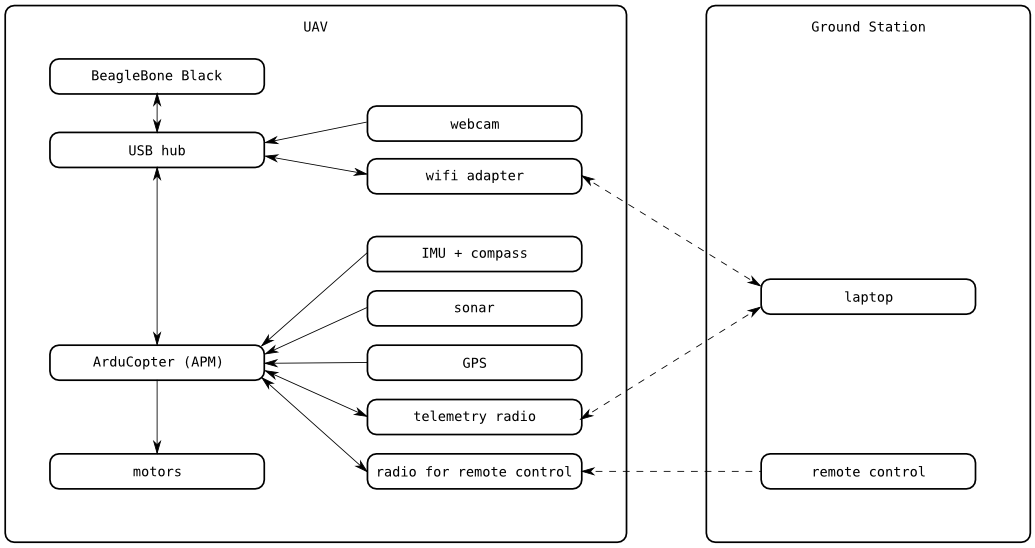
\includegraphics[width=0.9\textwidth]{images/architecture.png}
\caption{
    Architecture of our automated landing system. We use inexpensive
    off-the-shelf hardware. The laptop and remote control are for
    monitoring and emergency takeover by a human pilot. All the
    computation is performed onboard the UAV.
}
\label{fig:hardware-arch}
\end{figure}

\begin{figure}[h!]
\centering
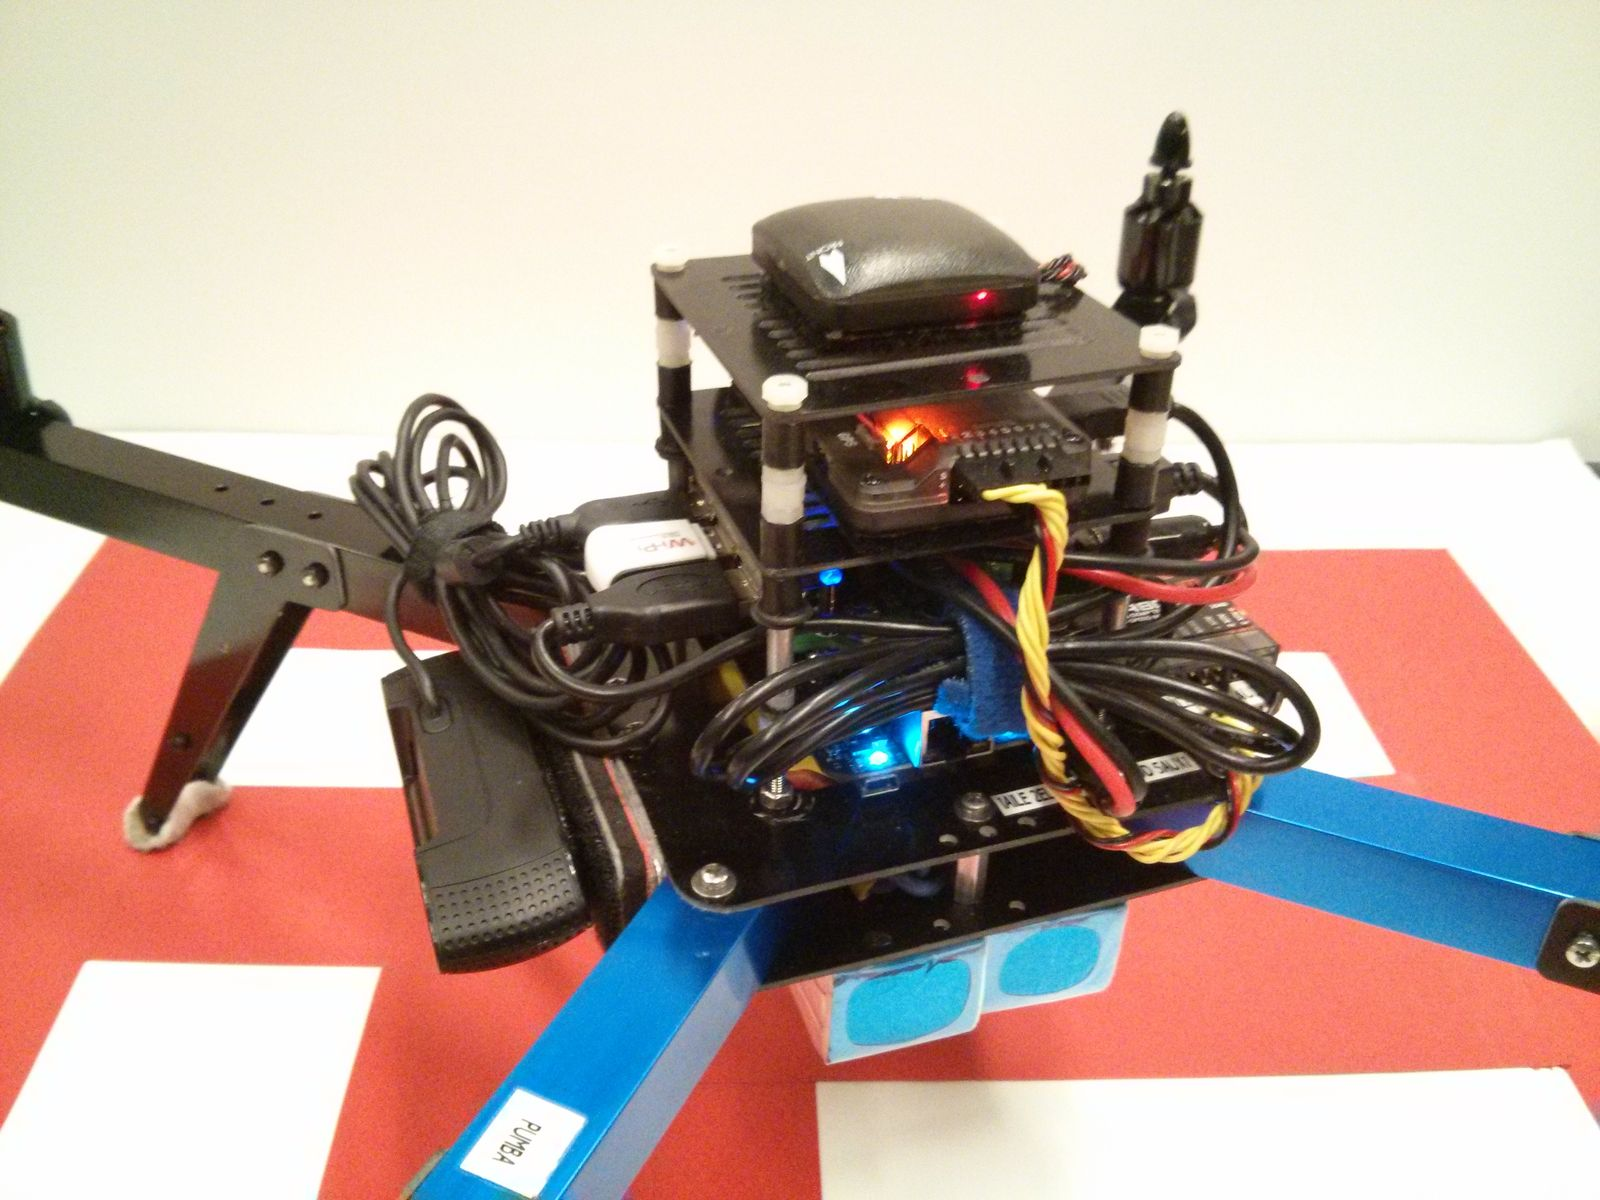
\includegraphics[width=0.85\textwidth]{images/hardware.jpg}
\caption{
    Our hardware stack fully assembled. From bottom to top: batteries,
    BeagleBone embedded computer, USB hub with Wi-Fi adapter, 3D
    Robotics autopilot with embedded sensors, GPS module. The
    webcam is on the left, and the radio for the remote control is on
    the right. Total weight excluding batteries is 1.35 kg.
}
\label{fig:hardware-photo}
\end{figure}

\begin{figure*}[h]
    \centering
    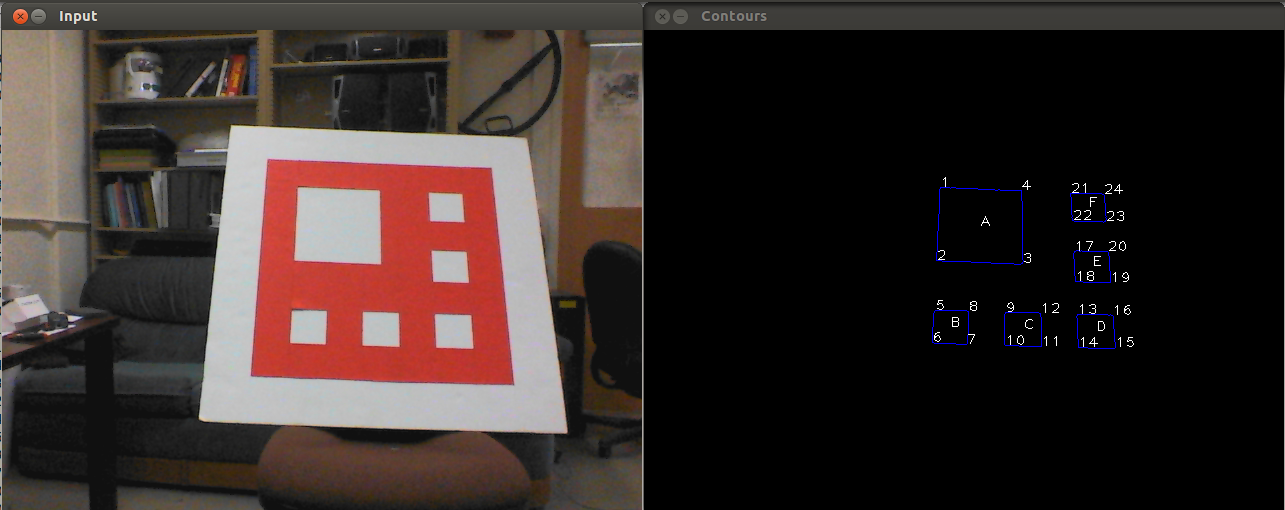
\includegraphics[width=\textwidth]{images/corners.png}
    \caption{
        Left: Design of our landing platform.
        Right: Output of the corner detector (24 points, in order).
    }
    \label{fig:corners}
\end{figure*}

\begin{figure}
    \begin{minipage}{0.5\textwidth}
        \centering
        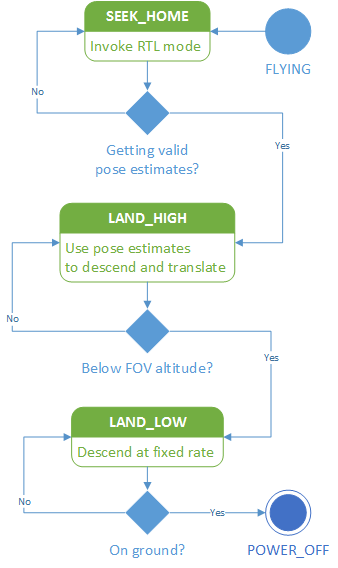
\includegraphics[width=0.9\linewidth]{images/statediagram.png}
        \caption{State diagram of our landing controller.}
        \label{fig:statediagram}
    \end{minipage}% this comment necessary, otherwise extra newline treated as space
    \begin{minipage}{0.5\textwidth}
        \centering
        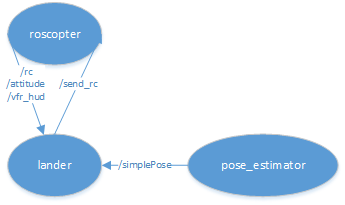
\includegraphics[width=0.9\linewidth]{images/rosnodes.png}
        \caption{ROS nodes and topics for exchanging messages.}
        \label{fig:rosnodes}
        \vspace{2cm}
        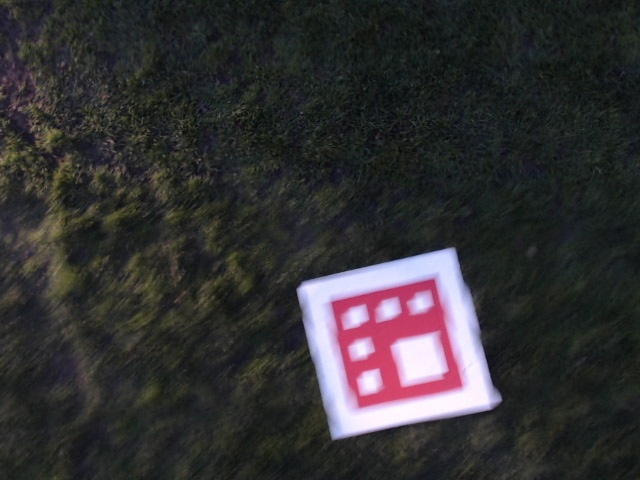
\includegraphics[width=0.9\linewidth]{images/badimage.jpg}
        \caption{An image where pose estimation fails.}
        \label{fig:badimage}
    \end{minipage}
\end{figure}

\end{document}
